\documentclass[11pt,a4paper]{article}
\usepackage[a4paper,margin=0.85in]{geometry}
\usepackage{amsmath,amssymb,amsthm}
\usepackage{booktabs,longtable,array}
\usepackage{graphicx}
\usepackage{float}
\usepackage{placeins}
\usepackage{caption}
\usepackage{lmodern}
\usepackage{microtype}
\usepackage[hidelinks]{hyperref}
\usepackage{xurl}

\hypersetup{
  pdftitle={Supplementary Information for Conditional validity of quantum event classifiers under collider systematics and quantum estimation uncertainty},
  pdfauthor={Roberto Fernandez-Barrios, Iker Pastor-Lopez, Asier Gonzalez-Santocildes, Pablo Garcia Bringas},
  pdfsubject={Supplementary Information submitted to npj Quantum Information}
}

\captionsetup{justification=raggedright,singlelinecheck=false}

\graphicspath{{../../results/figures/}}
\renewcommand{\thefigure}{S\arabic{figure}}
\renewcommand{\thetable}{S\arabic{table}}
\renewcommand{\thesection}{S\arabic{section}}
\setcounter{figure}{15}

\title{Supplementary Information for\\
\emph{Conditional validity of quantum event classifiers under collider
systematics and quantum estimation uncertainty}}
\author{Roberto Fern\'andez-Barrios\textsuperscript{1,*},
Iker Pastor-L\'opez\textsuperscript{1}\\
Asier Gonz\'alez-Santocildes\textsuperscript{1},
Pablo Garc\'ia Bringas\textsuperscript{1}\\[0.6em]
\small\textsuperscript{1}Faculty of Engineering, University of Deusto,
Avda. de las Universidades 24, 48007 Bilbao, Spain\\
\small\textsuperscript{*}Corresponding author:
\href{mailto:roberto.fernandez.b@deusto.es}{roberto.fernandez.b@deusto.es}}
\date{2026}

\begin{document}
\maketitle

\noindent\textbf{Scope of statistical guarantees.} Theorem 1's anytime-valid
error control applies to each fixed I2 label-stream claim, conditional on the
frozen finite audit population under the declared with-replacement sampling
protocol. I3 profile-likelihood and auxiliary-information procedures are
separately coverage-gated. The CMS and other empirical ledgers use their own
calibrated tests and information constraints and do not inherit Theorem 1
automatically.

This supplement gives the full algebra behind the formal results, the
registered-falsifier and correction trail, and extended numerical tables.
Every numerical table is a transcription or an explicitly identified
summary of the immutable JSON artifact named in its caption. Superseded
first-run tables remain in the repository under \texttt{*\_v1\_*.json}.

\section{Formal details}

\subsection{Exact weighted anytime-valid certification}
\label{supp:weighted}

Condition on a frozen finite audit population and a scalar $w_{\max}$ fixed
before the random audit order. For IID with-replacement labeled draws
$(c_i,u_i)$, with $c_i\in\{0,1\}$, $u_i\in[0,w_{\max}]$, $E[u]>0$, and
$R=E[uc]/E[u]$, fix $\tau\in[0,1]$ before observing the audit label stream and define
\[
 Z_i(\tau)=\frac{u_i(c_i-\tau)+\tau w_{\max}}{w_{\max}}.
\]
Because $u_i(c_i-\tau)$ lies between $-\tau w_{\max}$ and
$(1-\tau)w_{\max}$, $Z_i(\tau)\in[0,1]$. Moreover,
\[
 E[Z(\tau)]\geq\tau
 \iff E[u(c-\tau)]\geq0
 \iff E[uc]\geq\tau E[u]
 \iff R\geq\tau.
\]
Equivalently,
\[
 E[Z(\tau)]-\tau=\frac{E[u]}{w_{\max}}(R-\tau).
\]
The reduction is therefore exact. If $(L_n,U_n)$ is any level
$1-\alpha$ confidence sequence for the mean of $Z$, then on its
time-uniform coverage event $L_n\geq\tau$ implies $R\geq\tau$ at every
$n$. Thus
\[
 P\{\exists n:\text{SUPPORTED and }R<\tau\}\leq\alpha
\]
under arbitrary stopping; symmetrically,
$P\{\exists n:\text{REFUTED and }R\geq\tau\}\leq\alpha$. Both kinds of
incorrect decisive verdict are contained in the same two-sided CS coverage
failure, so their union for this fixed claim is also bounded by $\alpha$.
Setting $u\equiv1$ and $w_{\max}=1$ recovers
the unweighted construction. Weighting changes the variance and hence
the stopping time, but adds no validity slack. Labeling reveals $(y_i,w_i)$
and therefore $u_i=w_i$, $w_i1[y_i=1]$, or $w_i1[y_i=0]$ as appropriate;
event-wise weights remain unavailable to I1. The data-curation layer supplies
only the single global scalar bound before sampling, not row weights or class
labels; this does not enlarge I1 with event-level information. Both classes have positive
archived weight mass, establishing $E[u]>0$ for the class-conditional cases.
The multiplier 2.05 covers the largest admissible compound scale
$2.0\times1.01=2.02$.

This guarantee is per fixed claim and simultaneous only over its labeling
times/stopping rules. It is not FWER or simultaneous control over thresholds,
models, or environments; selecting $\tau$ or a claim after labels requires a
separate multiplicity construction. Time-uniformity also does not validate
arbitrary adaptive row selection. E07 instead uses a score-based proposal
fixed before labels and bounded importance weights.
The contribution claimed here is this exact fixed-$\tau$ ratio reduction and
its integration with the information-conditional auditor, not priority over
importance-weighted, self-normalized or adaptive-data confidence sequences;
the directly relevant off-policy literature is cited in the main manuscript.

\subsection{Information-set boundary for weight-only nuisances}
\label{supp:weight-only}

I1 is the fixed-size or count-conditioned feature experiment
$\mathcal O_1^{(n)}=(X_1,\ldots,X_n)\mid N=n$; it excludes $N$, exposure,
yields and event weights. If a weight-only nuisance satisfies
\[
 P_\theta(X_1,\ldots,X_n\mid N=n)=P_0(X_1,\ldots,X_n\mid N=n),
\]
every I1 statistic has the same sampling law. At I2 the simulated protocol
reveals a binary signal/background label and nominal weight for each queried
draw. The label does not reveal the background process category. If the joint
law of $(X,Y,w^{(0)})$ remains unchanged while the nuisance-dependent category
or true weight $w^{(\theta)}$ is hidden, the same indistinguishability result
holds. A level-$\alpha$ test then has power equal to its actual size and hence
at most $\alpha$; under the fail-closed policy, affected rate and true-weighted
claims remain UNRESOLVED.

This statement is deliberately limited to the declared experiment. The full
observable collider experiment may instead contain
$P_\theta(N,X_1,\ldots,X_N)$. At I3 a control-region count
$N\sim\operatorname{Poisson}(\lambda(\theta))$ with
$\lambda(\theta)\ne\lambda(0)$ changes that law and restores nontrivial power.
The restoration is quantitative rather than absolute:
template variance
\[
 \sigma_c^2=\sum_g(\operatorname{relerr}_g\lambda_g)^2
\]
sets the resolution scale. This is why the template-statistics-aware E14
fit identifies the ttbar rate only to approximately $\pm10\%$ and leaves
tighter claims unresolved.

\subsection{Random deployments and verdict stability}
\label{supp:random-deployments}

Let $\omega$ denote the finite-shot or hardware realization and
$\widetilde f_\omega$ the resulting refit, recalibration, and threshold.
If, conditional on $\omega$, the audit stream remains IID and disjoint from
training, calibration, and threshold selection, and the audit controls false certification,
\[
 P(\text{false certification}\mid\omega)\leq\alpha,
\]
then the tower property gives marginal control for both the
deployment-relative and ideal-anchored claim classes:
\[
 P(\text{false certification})
 =E_\omega[P(\text{false certification}\mid\omega)]\leq\alpha.
\]

For signed target and source movements $\Delta M_T$ and $\Delta M_S$, the
exact margin movements are $\Delta M_T$ for the ideal-anchored claim and
$\Delta M_T-\Delta M_S$ for the deployment-relative claim. Therefore
$|m^\star|>|\Delta M_T|$ or, respectively,
$|m^\star|>|\Delta M_T-\Delta M_S|$ is sufficient to preserve the truth-sign;
failure of a sufficient condition gives no conclusion. For either claim
class, the corresponding sign-stability condition plus coverage of both CSs
plus resolution of both audits implies the same decisive verdict. Conditional
on a realization satisfying stability, two level-$\alpha$ audits obey
\[
 P\{V^\star\ne V(\omega),R^\star\cap R(\omega)\mid\omega\}\leq2\alpha
\]
by a union bound. Running each audit at $\alpha/2$ gives joint level-$\alpha$
control; no sharper dependence-based result is used. Coverage and resolution
alone are insufficient: $m^\star=0.05$, $\Delta M_T=-0.10$ yields opposite
truth signs and opposite perfectly covered verdicts. Failure does not force a
flip either: $\Delta M_T=+0.10$ violates the inequality but preserves the sign.
For weighted claims the
metric-scale margin is mapped to the certification scale by
$E[u]/w_{\max}$. Common-mode movement cancels from the
deployment-relative margin but not from the ideal-anchored margin.
Although the original E16 summary archived only $\Delta M_S$, the final
deterministic replay reconstructs $\Delta M_T$ and
$\Delta M_T-\Delta M_S$ from the frozen source/target rows and the exact
replayed raw and PSD-repaired deployments. It therefore instantiates both
sufficient conditions without new randomness or QPU jobs; the resulting
7,200-case evaluation and its conservative interpretation are reported in
Section~\ref{sec:prop4-instantiation} and
Table~\ref{tab:prop4-instantiation}.
This E16 use is retrospective: the target movements are reconstructed from the
frozen target population after the deployment is available. Proposition 3 is
a formal sufficient sign-stability condition, but this instantiation is a
diagnostic of observed deployment stability rather than an operational
pre-audit certificate. A holding condition is sufficient for truth-sign
stability; a failing condition does not predict a flip, and audit verdicts
remain coverage-conditioned.

\subsection{Pre-split component allocation for weighted balanced accuracy}

For $\mathrm{BA}_w=(\mathrm{TPR}_w+\mathrm{TNR}_w)/2\geq\tau_{\rm BA}$,
the mathematical construction can predeclare component thresholds $\tau_1,\tau_2$ satisfying
$(\tau_1+\tau_2)/2=\tau_{\rm BA}$ and error levels
$\alpha_1+\alpha_2=\alpha$. Each component uses the exact one-sample
reduction with a valid class-specific bound. The BA claim is
SUPPORTED only if both components are supported, REFUTED only if both are
refuted, and UNRESOLVED otherwise. If BA is false, at least one component
claim is false; certifying it requires a coverage violation. A union bound
therefore controls false certification at $\alpha$. The symmetric argument
controls false refutation. In the executed E13v2 battery, however, the class
maxima were calculated using labels from the complete frozen population.
It is therefore an oracle/benchmark diagnostic rather than an operational
I2 guarantee. Table~\ref{tab:e13v2} shows that even this favorable oracle
construction is information-limited by the benchmark's weighted signal
fraction; successful TNR resolutions are reported only in that diagnostic sense.

\section{Registered falsifiers and audit trail}

The count below is by \emph{unique registered falsifier arm}. The E15
calibration gate is one arm, although it rejected two successive invalid
implementations before the valid grid was allowed to run. This convention
reconciles the nine-arm tally with the two gate interventions.

\footnotesize
\begin{longtable}{@{}>{\raggedright\arraybackslash}p{0.10\linewidth}>{\raggedright\arraybackslash}p{0.23\linewidth}>{\raggedright\arraybackslash}p{0.25\linewidth}>{\raggedright\arraybackslash}p{0.32\linewidth}@{}}
\caption{All nine registered falsifier arms that fired. Frozen conditions and consequences are recorded in \texttt{docs/experiment\_registry.md}.}\label{tab:falsifiers}\\
\toprule
Arm & Frozen condition & Observed firing & Consequence obeyed \\
\midrule
\endfirsthead
\toprule
Arm & Frozen condition & Observed firing & Consequence obeyed \\
\midrule
\endhead
E02R & TES sign pattern fails multi-seed replication & Up-shift monotonicity in only 2/5 seeds & Down-shift retained provisionally within-world; E17 later withdrew the directional cross-world claim. \\
E12(e) & Two flagship decoupling cells fail to reproduce & Diboson flagship cells stayed nominal-like in the fresh world & Normalization-collapse statement scoped to signal-region composition; failing registered cells kept. \\
E14 v1 & Control-region interval coverage below nominal & Pure-Poisson fit gave ttbar bias $+0.07$ and zero coverage & Run blocked; template-statistics likelihood registered, then rerun as v2. \\
E15 gate & Nominal L2 coverage outside $0.6827\pm0.02$ & Conditional-ensemble and numerical-conditioning implementations each failed & Both grids blocked; ensemble semantics and optimizer fixed before any shifted claim. \\
E17(b) & Degradation signs fail across additional worlds & One world improved QK under combo by 0.009; another under TES-down by 0.005 & Cross-world degradation claim withdrawn. \\
E08v2(a) & Corrected counting coverage outside the nominal band & One-draw corrected coverage $0.9916$--$1.000$ & Arm blocked and bounded multi-draw E08v3 registered. \\
E08v2(b) & Independent-template flagship L2 coverage $<0.633$ & Coverage 0.000 versus shared 0.7188 & ``Profiling restores validity'' made explicitly shared-simulation-conditional. \\
E08v3(a) & Marginal symmetric-BB coverage outside $0.6827\pm0.06$ for at least two gated models & All three gated models overcovered, 0.7513--0.8284 & Calibration-restoration claim withdrawn; conservative direction reported. \\
E13v2(b) & All true benchmark BA claims unresolved by 5,000 labels & TPR component 0/200 resolutions in every cell & BA path published as information-limited; TNR success and mechanism reported separately. \\
\bottomrule
\end{longtable}
\normalsize
\FloatBarrier

\begin{table}[H]
\centering
\small
\caption{Audit-trail summary. The full findings and dispositions are in \texttt{docs/audits/}.}
\label{tab:audit-trail}
\begin{tabular}{>{\raggedright\arraybackslash}p{0.19\linewidth}>{\raggedright\arraybackslash}p{0.20\linewidth}>{\raggedright\arraybackslash}p{0.51\linewidth}}
\toprule
Audit & Scope & Material effect \\
\midrule
Pre-campaign, 2026-08-11 & All E00--E11 code, tables, splits, and governance & Seven design constraints frozen before E12--E16: archived row indices, role separation, post-selection sensor validation, an independent floor, independent quantum-noise streams, a typed deployment snapshot, and weighted estimands. No prior headline invalidated. \\
Post-campaign, 2026-08-11 & E12--E16, E04v3, E11v2; 172 registry values and about 178 manuscript claims & E13 nominal-weight estimand fixed and rerun; E15 gate rejected two implementations; E16 dual accounting added; E12 normalization reading corrected; all superseded tables retained. \\
Pre-submission, 2026-08-12 & Extension runners, figure scripts, and line-by-line formal proofs & Two HIGH findings fixed: JES tracking scoped and disclosed; E19 weighted estimand corrected and rerun. Proposition 4 gained its coverage-event and scale-bridge qualifiers. Eight LOW findings were fixed, completed, disclosed, or documented. \\
F8.2, 2026-08-12 & Final LaTeX, supplement, number trace, semantic equivalence, rendered PDFs & E08v3 bias range corrected from $+6.1$ to the archived $+7.5$ endpoint; the nine-arm counting convention made explicit. \\
Final mathematical/editorial, 2026-08-12 & Proposition 2, Theorem 1, Proposition 4, Contributions 2/3, E17, figures, and three independent adversarial reviews & Claims were restricted to their exact mathematical and evidential scope: per-claim rather than family-wise control; finite-population-conditional weight bounds; conditional Proposition 4 with empirical flips separated; joint nuisance-representability/template-quality limits; no new experiment or result. \\
Senior-author pre-submission, 2026-08-13 & Observable experiments, Proposition 4, weighted-inference literature, E16 deployment unit, C2 narrative, CMS wording and concision & Added the missing sign-stability premise and counterexample; separated feature-conditioned evidence from counts; reanalyzed all 30 existing E16 deployments without new runs; retired IID environment $p$-values; updated related-manuscript status and reduced audit-history prose in the main paper. \\
Final pre-submission patch, 2026-08-31 & Primary literature, novelty claims, abstract hierarchy, methods, supplement, release metadata and rendered artifacts & Added the closest competitive work, removed priority language, made Contribution 3 deployment semantics primary, expanded protocol detail, and synchronized editorial/release records. No experiment, dataset, model, configuration or primary result changed. \\
Final technical PSD audit, 2026-08-31 & The 30 frozen E16 deployments, LIBSVM semantics, hardware-entry provenance and sealed-role wording & Deterministically replayed every raw deployment, measured the complete training-Gram spectra, applied one declared minimum-diagonal-loading sensitivity, and classified the result \textsc{PSD-sensitive-but-scoped}. No new Gram realization, seed, sample or QPU job was generated. \\
Mechanistic-clarity / derived-analysis patch, 2026-09-01 & The 30 frozen E16 deployments and their loaded counterparts, the Proposition-3 instantiation, the E13/E19 weighted audits, C2/C3 framing & Deterministic counterfactual stage decomposition after exact endpoint reproduction (predeclared classification \textsc{mixed}: recalibration generates the far-margin flips, threshold refreezing partly compensates); Proposition 3 stratified by margin; weight-bound conservatism measured on identical streams; plain-language abstract; adverse independent-template result leads Contribution 2; editorial corrections. No new randomness, seed, sample, model, repair, likelihood or QPU job. 0.3.7: regime-specific C3 wording only. \\
\bottomrule
\end{tabular}
\end{table}
\FloatBarrier

\section{Extended numerical results}

\subsection{Inference sensitivity (E15)}

Table~\ref{tab:e15sens} reports the local slope at the nominal point,
averaged over the five injected $\mu$ values. L1 is the counting
estimator, L2 the complete profile, and L3 the profile with the shifted
family omitted. Only the three models that passed the nominal L2 gate are
shown. Units are $\mu$ per nuisance unit: per standard deviation for TES
and JES, per GeV for soft-MET, and per unit scale for the normalization
families.

The archived initial global optimizer-success flag is conservative and falls
as low as 0.382. Analytic gradients, multi-start fitting, a
monotone lower-minimum safeguard, and the nominal coverage gate support the
reported solutions but do not prove global optimization in every shifted cell.

\footnotesize
\begin{longtable}{llrrrr}
\caption{E15 local sensitivity and nuisance tracking. Source: \texttt{results/tables/E15\_sensitivity.json}.}\label{tab:e15sens}\\
\toprule
Family & Model & L1 slope & L2 slope & L3 slope & L2 tracking \\
\midrule
\endfirsthead
\toprule
Family & Model & L1 slope & L2 slope & L3 slope & L2 tracking \\
\midrule
\endhead
TES & QK-SVC & 9.8095 & 0.4092 & 7.1213 & 0.9970 \\
TES & RBF-SVC & 10.3065 & 0.2269 & 8.6641 & 0.9986 \\
TES & XGBoost & 5.4959 & 0.1031 & 4.7948 & 0.9938 \\
JES & QK-SVC & 3.6530 & -0.2033 & 5.1238 & 0.9813 \\
JES & RBF-SVC & 2.7528 & -0.1096 & 5.7069 & 0.9901 \\
JES & XGBoost & 1.7328 & 0.0121 & 1.1957 & 0.7116 \\
soft-MET & QK-SVC & -0.0812 & -0.2126 & 6.5142 & 0.2497 \\
soft-MET & RBF-SVC & 0.7731 & -0.0496 & 3.0473 & 0.2511 \\
soft-MET & XGBoost & 0.7305 & -0.4605 & -1.5627 & 0.5001 \\
ttbar scale & QK-SVC & 49.7510 & 0.5175 & -0.7125 & 1.0040 \\
ttbar scale & RBF-SVC & 54.0570 & -1.1795 & -4.0830 & 0.9915 \\
ttbar scale & XGBoost & 12.7935 & -0.0220 & 9.0305 & 0.9895 \\
diboson scale & QK-SVC & 4.7626 & 0.0834 & 0.5676 & 0.9900 \\
diboson scale & RBF-SVC & 4.3356 & 0.2769 & 1.0303 & 0.9869 \\
diboson scale & XGBoost & 0.9981 & -0.0065 & 0.4824 & 1.0006 \\
background scale & QK-SVC & 270.1200 & -30.9900 & 222.4700 & 1.0000 \\
background scale & RBF-SVC & 397.2600 & 34.5600 & 823.4100 & 0.9800 \\
background scale & XGBoost & 101.8800 & -5.3900 & -3.6800 & 1.0000 \\
\bottomrule
\end{longtable}
\normalsize

\subsection{Fresh-world validity and stopping-time efficiency}

\begin{table}[H]
\centering
\small
\caption{Fresh-world validity replication. Source: \texttt{results/tables/E19\_fresh\_world\_validity.json}; the false-refutation counts documented in the registered status agree with the rates stored in the table.}
\label{tab:e19}
\begin{tabular}{lrrr}
\toprule
Accounting & False certification & False refutation & Historical heuristic gate \\
\midrule
Unweighted, non-vetoed & 11/3,060 = 0.359\% & 1/11,980 = 0.008\% & 6.182\% \\
Unweighted, all streams & 11/7,700 = 0.143\% & 1/11,980 = 0.008\% & 6.182\% \\
Weighted, nominal weights & 6/7,980 = 0.075\% & 4/11,700 = 0.034\% & 5.732\% \\
\bottomrule
\end{tabular}

\vspace{0.5em}
\parbox{0.94\linewidth}{\footnotesize All 12 archived model--environment
score comparisons were byte-identical before auditing. The weighted bound
was $w_{\max}=7.22421\times2.05=14.80963$. The corrected nominal-weight
estimand is invariant across all 12 weight-only environments.}
\parbox{0.94\linewidth}{\footnotesize The final column retains the historical
$\alpha+3\sigma$ implementation gate. It used a binomial heuristic over pooled,
correlated stream counts: streams share audit draws, deployments, claim grids
and thresholds. It is therefore not interpreted as an IID sampling standard
error or confidence boundary. It is retained only as a historical
implementation-falsifier threshold. Formal validity follows from the
per-claim confidence-sequence result; the pooled empirical rates are
descriptive implementation diagnostics, not a proof of the theorem or
family-wise error control.}
\end{table}

\begin{table}[H]
\centering
\small
\caption{Audit-label draw-budget price relative to the Wald information
yardstick. Sampling is with replacement, so $n^*$ is a labeled-observation
budget rather than a unique-event label cost. Source:
\texttt{results/tables/E06\_nstar\_efficiency.json}.}
\label{tab:nstar}
\begin{tabular}{lrrrr}
\toprule
Subset & Cells & Q25 & Median & Q75 \\
\midrule
All resolved cells & 518 & 1.56 & 2.07 & 2.97 \\
Margin $[0.01,0.02)$ & 95 & 2.82 & 3.35 & 3.85 \\
Margin $[0.02,0.04)$ & 95 & 2.62 & 3.19 & 3.66 \\
Margin $[0.04,0.08)$ & 164 & 1.63 & 1.98 & 2.38 \\
Margin $\geq0.08$ & 164 & 1.25 & 1.46 & 1.72 \\
Certification direction & 487 & 1.54 & 1.99 & 2.78 \\
Refutation direction & 31 & 3.12 & 3.34 & 3.65 \\
\bottomrule
\end{tabular}
\end{table}

\subsection{Quantum-estimation diagnostics (E16)}

\begin{figure}[H]
\centering
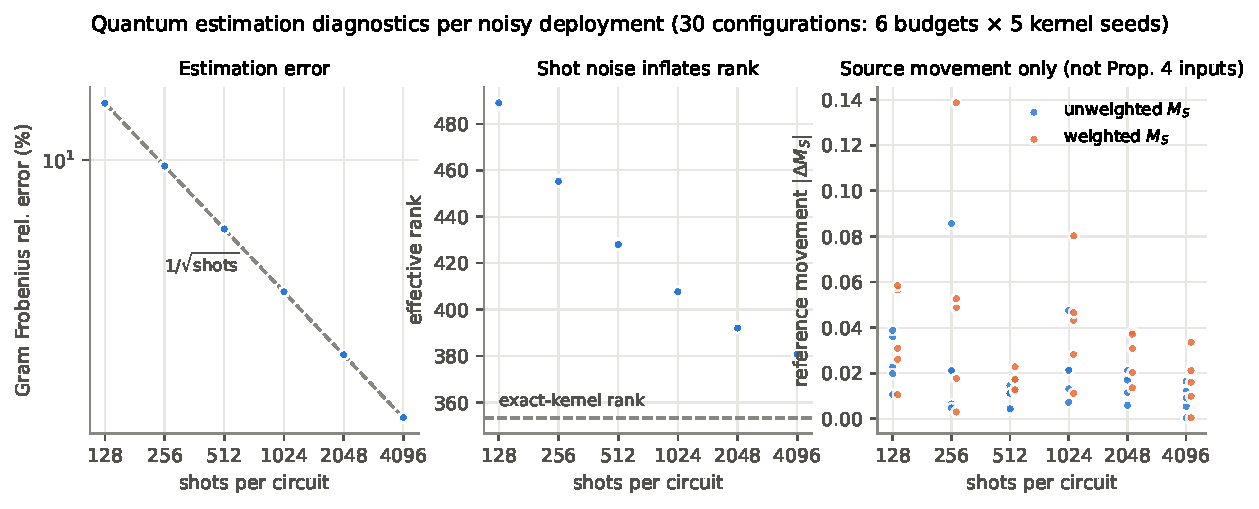
\includegraphics[width=0.98\linewidth]{figS16_estimation_diagnostics.pdf}
\caption{Per-configuration diagnostics for all 30 noisy deployments:
relative Frobenius error, effective-rank inflation, and source-reference
movement $|\Delta M_S|$. The primary artifact plotted only source movement;
the final deterministic raw/PSD replay reconstructs
$\Delta M_T$ and $\Delta M_T-\Delta M_S$ and instantiates Proposition 3 in
Table~\ref{tab:prop4-instantiation}. Sources:
\texttt{results/tables/E16\_quantum\_uncertainty.json} and
\texttt{results/tables/E16\_proposition4\_instantiation.json}. The archived
artifact names retain the historical identifier `proposition4' used before the
formal results were renumbered; the corresponding formal result is
Proposition 3.}
\label{fig:s16}
\end{figure}

The primary replication unit is the independently sampled noisy-kernel
realization, five per shot budget. Within a deployment, 200 far, 170 moderate
and 230 near claims share the Gram matrix, refit, calibration, threshold and
audit streams; their count is not an IID sample size. Audit streams are paired
across deployments, so comparisons also share common random numbers. The far ideal-anchored deployment means are
20.8, 17.7, 0.9, 11.9, 5.8 and 0.4\%; the intermediate values are each
dominated by one or two deployments, so the sequence reflects deployment
heterogeneity and outlier sensitivity rather than a budget trend. At the endpoints the sample SDs are 19.9 and 0.65\%, ranges are
0--44 and 0--1.5\%, and leave-one-deployment-out means are 15--26 and
0.13--0.50\%. These are descriptive dispersion and sensitivity summaries, not
population confidence intervals. Five deployments per budget permit only a
descriptive characterization of the observed realizations; no population
trend or equivalence claim is made.
All far-margin deployment-relative claims in this evaluated grid are true and
remain SUPPORTED in every raw and PSD-repaired realization. Consequently, the
zero far-margin flip rate demonstrates stability of clearly true/supported
claims only; this grid contains no false far-margin deployment-relative claim
with which to assess refutation stability.

\clearpage
\begin{table}[H]
\centering
\scriptsize
\setlength{\tabcolsep}{3pt}
\caption{E16 results by noisy-kernel deployment. Rates are percentages of the
correlated claims within that deployment, not independent replication. ``Fixed''
is ideal-anchored and ``own'' is deployment-relative. Source:
\texttt{results/tables/E16\_quantum\_uncertainty.json}; derived deployment
summary: \texttt{results/tables/E16\_deployment\_level.json}.}
\label{tab:e16}
\begin{tabular}{rrrrrrrrr}
\toprule
Shots & Seed & Frob.\ (\%) & AUC & \multicolumn{2}{c}{Far flips} & \multicolumn{2}{c}{Moderate flips} & Near abst. \\
 & & & & fixed & own & fixed & own & own \\
\midrule
128 & 1 & 13.64 & 0.8336 & 0.0 & 0.0 & 52.3 & 14.7 & 95.7 \\
128 & 2 & 13.69 & 0.8311 & 11.5 & 0.0 & 74.7 & 15.9 & 94.8 \\
128 & 3 & 13.66 & 0.8338 & 40.0 & 0.0 & 80.0 & 14.1 & 93.9 \\
128 & 4 & 13.66 & 0.8377 & 44.0 & 0.0 & 78.8 & 18.2 & 93.0 \\
128 & 5 & 13.67 & 0.8384 & 8.5 & 0.0 & 71.2 & 15.9 & 92.6 \\
256 & 1 & 9.67 & 0.8361 & 0.0 & 0.0 & 50.0 & 18.2 & 92.2 \\
256 & 2 & 9.66 & 0.8331 & 0.0 & 0.0 & 34.1 & 11.8 & 93.9 \\
256 & 3 & 9.67 & 0.8278 & 0.0 & 0.0 & 50.0 & 12.3 & 92.2 \\
256 & 4 & 9.65 & 0.8364 & 0.0 & 0.0 & 32.9 & 16.5 & 90.4 \\
256 & 5 & 9.66 & 0.8436 & 88.5 & 0.0 & 80.0 & 21.8 & 95.7 \\
512 & 1 & 6.85 & 0.8307 & 2.0 & 0.0 & 62.4 & 9.4 & 96.1 \\
512 & 2 & 6.84 & 0.8394 & 0.0 & 0.0 & 30.0 & 10.6 & 91.3 \\
512 & 3 & 6.83 & 0.8480 & 1.0 & 0.0 & 57.6 & 12.3 & 90.9 \\
512 & 4 & 6.83 & 0.8486 & 0.0 & 0.0 & 30.6 & 10.6 & 93.5 \\
512 & 5 & 6.83 & 0.8478 & 1.5 & 0.0 & 57.6 & 14.7 & 90.9 \\
1024 & 1 & 4.83 & 0.8385 & 0.0 & 0.0 & 49.4 & 15.3 & 90.9 \\
1024 & 2 & 4.83 & 0.8338 & 0.0 & 0.0 & 51.2 & 12.9 & 90.9 \\
1024 & 3 & 4.84 & 0.8381 & 0.0 & 0.0 & 47.1 & 11.8 & 93.9 \\
1024 & 4 & 4.83 & 0.8381 & 59.0 & 0.0 & 80.0 & 15.9 & 93.0 \\
1024 & 5 & 4.84 & 0.8385 & 0.5 & 0.0 & 45.3 & 10.0 & 91.3 \\
2048 & 1 & 3.42 & 0.8366 & 0.0 & 0.0 & 32.9 & 10.0 & 94.8 \\
2048 & 2 & 3.42 & 0.8460 & 0.0 & 0.0 & 49.4 & 10.0 & 93.0 \\
2048 & 3 & 3.42 & 0.8469 & 3.0 & 0.0 & 61.2 & 12.9 & 90.4 \\
2048 & 4 & 3.42 & 0.8496 & 14.0 & 0.0 & 73.5 & 11.2 & 96.5 \\
2048 & 5 & 3.42 & 0.8428 & 12.0 & 0.0 & 74.7 & 11.2 & 94.8 \\
4096 & 1 & 2.42 & 0.8409 & 0.0 & 0.0 & 39.4 & 4.7 & 93.0 \\
4096 & 2 & 2.42 & 0.8444 & 0.0 & 0.0 & 3.5 & 5.3 & 91.7 \\
4096 & 3 & 2.42 & 0.8357 & 1.5 & 0.0 & 56.5 & 10.6 & 94.8 \\
4096 & 4 & 2.42 & 0.8373 & 0.0 & 0.0 & 48.8 & 8.2 & 92.2 \\
4096 & 5 & 2.42 & 0.8400 & 0.5 & 0.0 & 53.5 & 4.7 & 93.5 \\
\bottomrule
\end{tabular}
\end{table}

\begin{table}[H]
\centering
\scriptsize
\setlength{\tabcolsep}{2.5pt}
\caption{Post-hoc E16 PSD sensitivity prompted by the final technical audit.
Each row summarizes five deterministically replayed frozen deployments. Flip
entries are mean far-margin percentages relative to the ideal exact-kernel
deployment; ``dep.'' uses each realization's refrozen source reference and
``ideal'' uses the fixed ideal reference. Minimum diagonal loading preserves
every off-diagonal and cross-Gram estimate. Source:
\texttt{results/tables/E16\_psd\_sensitivity.json}.}
\label{tab:e16-psd}
\begin{tabular}{rrrrrrrrrr}
\toprule
Shots & $n$ & med. $\lambda_{\min}$ & worst $\lambda_{\min}$ & med. $n_-$ & max $n_-$ & dep. raw & dep. PSD & ideal raw & ideal PSD \\
\midrule
128  & 5 & $-1.930$ & $-1.939$ & 580 & 580 & 0.0 & 0.0 & 20.8 & 31.5 \\
256  & 5 & $-1.325$ & $-1.333$ & 531 & 532 & 0.0 & 0.0 & 17.7 & 40.7 \\
512  & 5 & $-0.936$ & $-0.966$ & 489 & 490 & 0.0 & 0.0 & 0.9 & 25.1 \\
1024 & 5 & $-0.655$ & $-0.657$ & 449 & 450 & 0.0 & 0.0 & 11.9 & 3.0 \\
2048 & 5 & $-0.448$ & $-0.457$ & 412 & 413 & 0.0 & 0.0 & 5.8 & 6.9 \\
4096 & 5 & $-0.313$ & $-0.319$ & 379 & 380 & 0.0 & 0.0 & 0.4 & 0.3 \\
\bottomrule
\end{tabular}
\end{table}

All 30 raw $2000\times2000$ training Grams are indefinite under the declared
negative-mode tolerance $10^{-10}\max(1,|\lambda_{\max}|)$. Across budgets,
the median negative spectral-mass fraction falls from 13.59\% to 2.14\%, while
$\lambda_{\max}$ remains approximately 201.2; the positive-only condition
number ranges from $8.8\times10^4$ to $6.4\times10^7$ and is descriptive only
because the raw matrices are indefinite. The historical finite-shot pipeline
fits an SVC to each realized quantum-similarity matrix. Entry-wise finite-shot
estimation does not preserve positive semidefiniteness, so this RAW-INDEFINITE
fitted object is not interpreted as the standard convex RKHS SVM associated
with a PSD kernel.
The material far-margin changes are confined to the ideal-anchored magnitude:
they are substantial at 128--1024 shots, small at 2048 and negligible at 4096;
the deployment-relative far rate is unchanged at every budget.
LIBSVM can and did return a numerical solution when supplied each precomputed
raw matrix; indefiniteness alone also does not make its numerical deployment
meaningless.

The historical RAW-INDEFINITE pipeline remains primary. For the declared
sensitivity, each training Gram is converted in float64 as
$K_{\rm PSD}=K_{\rm raw}+\delta I$, where
$\delta=\max(0,-\lambda_{\min}+\epsilon)$ and
$\epsilon=10^{-10}\max(1,|\lambda_{\max}|)$ (approximately $2.01\times10^{-8}$
here). This is the minimum predeclared diagonal load up to the numerical
margin; it preserves all off-diagonal finite-shot estimates. The loaded
training block restores a convex precomputed-SVM training problem, but it is a
post-hoc regularized similarity matrix, not a normalized fidelity Gram: the
diagonal changes, source/target cross-Grams remain unchanged, and no global
Mercer extension is claimed. Each repaired deployment is then refitted,
Platt-recalibrated, threshold-refrozen and audited on exactly the same roles,
claim grids and paired audit streams. No Gram, sample, seed or QPU job is newly
drawn.

The PSD-repaired nominal-AUC means differ from raw by $+0.0051$ to $+0.0137$
across budgets; these changes are a sensitivity outcome, not a repair-selection
or performance claim. Raw-versus-repaired deployment-relative verdict-change
rates are zero in the far stratum, at most 19.9\% in moderate and 7.6\% in near;
ideal-anchored compositions move more strongly. Nevertheless, the observed
support stability of the evaluated true far-margin deployment-relative claims,
ideal-anchored heterogeneity,
outlier sensitivity and endpoint reduction all survive. The exact
deployment metrics, thresholds, target metrics, abstention, verdict
compositions and transitions are archived in the source JSON. The audit
verdict is therefore \textsc{PSD-sensitive-but-scoped}: Contribution 3's
qualitative statement survives, whereas its raw ideal-anchored percentages
must not be treated as repair-invariant.

\subsubsection{Deterministic retrospective instantiation of Proposition 3}
\label{sec:prop4-instantiation}

For the unweighted family, $M$ is mean correctness on the frozen source or
target rows; for the weighted family it is raw-physical-weighted mean
correctness on those rows. For each deployment $\omega$, the replay computes
$\Delta M_S=M_S(\tilde f_\omega)-M_S(f^\star)$ and
$\Delta M_T=M_T(\tilde f_\omega)-M_T(f^\star)$. The evaluated movement is
$\Delta M_T-\Delta M_S$ for deployment-relative claims and $\Delta M_T$ for
ideal-anchored claims. Every reconstructed threshold is interior to $[0,1]$,
and both exact margin identities have zero numerical residual, so all 7,200
condition cells are evaluable.

This is a retrospective diagnostic: $\Delta M_T$ and
$\Delta M_T-\Delta M_S$ require the frozen target rows and their labels/metrics
after deployment. It does not supply a prospective operational certificate
before target observation or audit. ``H'' remains a sufficient truth-sign
stability condition, whereas ``F'' does not predict a flip; verdict comparisons
remain conditioned on confidence-sequence coverage and resolution.

\begin{table}[H]
\centering
\small
\setlength{\tabcolsep}{4pt}
\caption{Proposition 3 instantiation. ``H'' and ``F'' mean that the strict
sufficient condition holds or fails; entries are verdict flip/no-flip counts
over the ten paired audit streams per condition cell. Cells and streams within
a deployment are correlated; the descriptive unit remains the deployment.
Source: \texttt{results/tables/E16\_proposition4\_instantiation.json}.}
\label{tab:prop4-instantiation}
\begin{tabular}{lrrrr}
\toprule
Cut & Condition cells & H (\%) & H: flip/no flip & F: flip/no flip \\
\midrule
Overall & 7,200 & 68.7 & 4,554 / 44,876 & 13,637 / 8,933 \\
RAW-INDEFINITE & 3,600 & 70.3 & 2,260 / 23,060 & 6,247 / 4,433 \\
PSD-repaired & 3,600 & 67.0 & 2,294 / 21,816 & 7,390 / 4,500 \\
Deployment-relative & 3,600 & 92.8 & 2,127 / 31,283 & 62 / 2,528 \\
Ideal-anchored & 3,600 & 44.5 & 2,427 / 13,593 & 13,575 / 6,405 \\
Far & 2,400 & 95.3 & 683 / 22,197 & 967 / 153 \\
Moderate & 2,040 & 70.0 & 2,955 / 11,325 & 4,112 / 2,008 \\
Near & 2,760 & 44.5 & 916 / 11,354 & 8,558 / 6,772 \\
\bottomrule
\end{tabular}
\end{table}

The inequality holds in 4,943/7,200 cells and preserves the truth sign in all
4,943, while 1,188 of the 2,257 failing cells also retain their sign. At audit
level, ternary verdict flips occur in 9.2\% of streams when the condition holds
and 60.4\% when it fails. Two condition-holding streams produce opposite
resolved verdicts; Proposition 3 bounds such events through confidence-sequence
coverage and does not assert deterministic verdict equality from the margin
inequality alone. The condition is therefore informative but conservative:
it is most useful for deployment-relative far/moderate cells and least often
satisfied for near ideal-anchored cells; it is sufficient rather than
necessary. This classification is
\textsc{informatively instantiated}, not an empirical general law or a set of
independent claim replications.

Table~\ref{tab:prop4-deployment-summary} changes the descriptive aggregation
unit from correlated cells/streams to the 30 noisy-kernel deployments. Each
deployment contributes 60 evaluable cells to every regime--semantics slice.
No population inference or independence assumption is added.

\begin{table}[H]
\centering
\scriptsize
\setlength{\tabcolsep}{3pt}
\caption{Deployment-level descriptive aggregation of Proposition 3. Each
column summarizes the 30 noisy-kernel deployments for one analysis slice;
each deployment contains 60 evaluable condition cells in that slice. Entries
are percentages shown as median [Q1, Q3] on the first line and min--max on the
second. Verdict-flip rates condition on the paired audit streams attached to H
or F cells; truth-sign rates are cell-level. The descriptive unit is the
noisy-kernel deployment, not the cell or audit stream. One RAW
deployment-relative deployment has no F cells, so its F-conditioned rates are
undefined and those two summaries use 29 deployments. Every H-conditioned
truth-sign flip rate is zero. Source:
\texttt{results/tables/E16\_proposition4\_deployment\_summary.json}.}
\label{tab:prop4-deployment-summary}
\resizebox{\textwidth}{!}{%
\begin{tabular}{lcccc}
\toprule
Statistic & RAW, deployment-relative & RAW, ideal-anchored & PSD, deployment-relative & PSD, ideal-anchored \\
\midrule
Evaluable cells & 60 & 60 & 60 & 60 \\
H cells (\%) & \shortstack{93.3 [92.1, 95.0]\\86.7--100.0} & \shortstack{42.5 [35.8, 57.9]\\8.3--96.7} & \shortstack{91.7 [90.4, 93.3]\\85.0--96.7} & \shortstack{41.7 [27.5, 50.8]\\8.3--86.7} \\
F cells (\%) & \shortstack{6.7 [5.0, 7.9]\\0.0--13.3} & \shortstack{57.5 [42.1, 64.2]\\3.3--91.7} & \shortstack{8.3 [6.7, 9.6]\\3.3--15.0} & \shortstack{58.3 [49.2, 72.5]\\13.3--91.7} \\
Verdict flips among H (\%) & \shortstack{5.8 [4.8, 7.3]\\2.8--9.4} & \shortstack{19.0 [4.7, 21.6]\\1.9--56.0} & \shortstack{7.1 [4.9, 8.2]\\3.1--12.0} & \shortstack{18.9 [5.9, 21.9]\\1.7--76.0} \\
Verdict flips among F (\%) & \shortstack{0.0 [0.0, 2.9]\\0.0--6.7} & \shortstack{62.2 [37.7, 76.9]\\0.0--91.6} & \shortstack{2.0 [0.0, 4.8]\\0.0--8.0} & \shortstack{58.7 [48.7, 88.8]\\7.5--91.8} \\
Truth-sign flips among F (\%) & \shortstack{50.0 [37.5, 66.7]\\0.0--75.0} & \shortstack{45.5 [31.4, 61.5]\\27.6--70.6} & \shortstack{40.0 [29.8, 50.0]\\16.7--75.0} & \shortstack{45.5 [34.9, 56.9]\\27.6--69.7} \\
\bottomrule
\end{tabular}%
}
\end{table}

Table~\ref{tab:prop3-stratification} stratifies the same 7,200 cells by the
magnitude of the ideal margin. The bins refine the registered far/moderate/near
strata and are descriptive. For ideal-anchored claims the HOLDS/FAILS
distinction remains informative within every bin: paired-stream flip rates are
2.7--38.7\% when the inequality holds and 63.8--100\% when it fails. For
deployment-relative claims the inequality fails only when
$|m^\star|<0.005$ (largest failing margin 0.0040), because the relevant
movement $\Delta M_T-\Delta M_S$ is itself small in E16 (median 0.0011,
maximum 0.0063 over both regimes); in that single bin the failing cells flip
less often (2.4\%) than the holding cells (4.9\%), so the same interpretation
is not supported for that class. Source and target movements are predominantly
common-mode, and the deployment-relative margin cancels most of the observed
deployment perturbation; the formal sufficient condition is general, but the
empirical deployment-relative stability observed here is largely explained by
this common-mode cancellation.

\begin{table}[H]
\centering
\small
\setlength{\tabcolsep}{4pt}
\caption{Proposition 3 instantiation stratified by ideal-margin magnitude
$|m^\star|$, pooled over the raw and PSD-sensitivity regimes. ``H''/``F'': the
strict sufficient inequality holds/fails; flip rates are ternary verdict flips
per paired audit stream. Cells and streams within a deployment are correlated
and no IID test is performed. Source:
\texttt{results/tables/E16\_prop3\_margin\_stratification.json}.}
\label{tab:prop3-stratification}
\begin{tabular}{llrrrr}
\toprule
Class & $|m^\star|$ & H cells & F cells & Flips H (\%) & Flips F (\%) \\
\midrule
deployment-relative & $[0,0.005)$ & 521 & 259 & 4.9 & 2.4 \\
deployment-relative & $[0.005,0.01)$ & 600 & 0 & 8.3 & -- \\
deployment-relative & $[0.01,0.02)$ & 720 & 0 & 15.9 & -- \\
deployment-relative & $[0.02,0.04)$ & 300 & 0 & 7.7 & -- \\
deployment-relative & $[0.04,0.08)$ & 600 & 0 & 0.0 & -- \\
deployment-relative & $\geq0.08$ & 600 & 0 & 0.0 & -- \\
ideal-anchored & $[0,0.005)$ & 28 & 752 & 6.8 & 63.8 \\
ideal-anchored & $[0.005,0.01)$ & 78 & 522 & 18.8 & 70.8 \\
ideal-anchored & $[0.01,0.02)$ & 218 & 502 & 38.7 & 65.1 \\
ideal-anchored & $[0.02,0.04)$ & 190 & 110 & 38.6 & 76.7 \\
ideal-anchored & $[0.04,0.08)$ & 504 & 96 & 10.4 & 84.1 \\
ideal-anchored & $\geq0.08$ & 584 & 16 & 2.7 & 100.0 \\
\bottomrule
\end{tabular}
\end{table}

\subsubsection{Stage decomposition of the frozen E16 deployments}
\label{sec:stage-decomposition}

To locate where the finite-shot perturbation is amplified, the 30 raw
deployments and their 30 minimum-diagonal-loading counterparts were replayed
deterministically from the frozen RNG schedule and evaluated at diagnostic
counterfactual stages: A, the ideal deployment; B0, the SVC refitted on the
realized training Gram but evaluated on the exact source/target cross-Grams
with the ideal Platt map and threshold; B, the realized decision function
(noisy fit and noisy cross-Grams) with the ideal Platt map and threshold; C,
the realized decision function with its deployment-specific Platt map and the
ideal probability threshold; and D, the archived full deployment with its own
refrozen threshold. Stages B0--C were never deployed; they are diagnostic
counterfactuals. Stage D reproduced every archived RAW primary summary and
every archived PSD-sensitivity summary exactly, and the movements
$\Delta M_S$ and $\Delta M_T$ matched the frozen Proposition-3 instantiation
with zero residual in all 3,600 cells, before any stage was interpreted. The
four increments of the source metric telescope exactly to the full movement;
the attribution is sequential and depends on the declared pipeline order
(fit, evaluation cross-Grams, calibration, operating threshold), and a
different order could redistribute it. The classification rule was fixed
before the replay: a stage group (model/ranking $=$ fit $+$ evaluation;
calibration; threshold) dominates a regime when both its share of the mean
absolute source-metric increment and its share of the positive far-margin
ideal-anchored flip increment are at least one half; the regime label
requires the unweighted and weighted families to agree, otherwise
\textsc{mixed}. No new randomness, seed, sample, model, threshold rule, PSD
repair or QPU job was introduced; the artifact is
\texttt{results/tables/E16\_stage\_decomposition.json}.

Table~\ref{tab:stage-decomposition} summarizes the stages. In the raw
pipeline the realized decision function keeps the ideal ranking moderately
well (median Spearman 0.92, Kendall 0.78 on \texttt{source\_val}; 0.95 and
0.84 for the fit-only stage) and changes nominal AUC by a median $+0.001$. The
increments of source unweighted accuracy have mean absolute values 0.0015
(fit), 0.0059 (evaluation), 0.0122 (calibration) and 0.0197 (threshold), i.e.\
shares 3.9, 15.1, 31.0 and 50.0\%; their medians are $-0.0009$, $-0.0041$,
$-0.0092$ and $+0.0090$, so the threshold step carries the largest absolute
movement but with the sign opposite to recalibration. Far-margin
ideal-anchored flips are 0.0, 0.2, 14.3 and 9.6\% at B0, B, C and D:
recalibration at the fixed probability threshold generates almost all of them
(99\% of the positive flip increment) and threshold refreezing removes part of
them. By the predeclared rule the raw regime is \textsc{mixed}. In the
loaded regime the fit-only stage already moves source accuracy by a median
$-0.053$ while AUC rises by a median 0.017 and ranking stability is unchanged:
diagonal loading rescales the decision function, so the ideal Platt map no
longer matches its scale. Recalibration and threshold refreezing then recover
most of the movement (far flips 60.3, 64.9, 31.4 and 17.9\%). The rule labels
that regime \textsc{model/ranking-dominated}, with the qualification that the
model-stage increment is a scale change rather than a ranking loss; the
overall classification is \textsc{mixed}, and no universal downstream
mechanism is claimed across kernel treatments. The metric that selects the
operating point is more stable than the audited estimands: at stage D the
weighted balanced accuracy moves by a median 0.007 in both regimes, against
0.014 (raw) and 0.015 (loaded) for unweighted accuracy and 0.024 and 0.029
for weighted accuracy, and it is the smaller movement in 25 of 30 raw and 28
of 30 loaded deployments. Source and target movements remain common-mode at
every stage (stage D: median $|\Delta M_T-\Delta M_S|$ of 0.0010 and 0.0012
against median $|\Delta M_T|$ of 0.014 and 0.013).

\begin{table}[H]
\centering
\scriptsize
\setlength{\tabcolsep}{3pt}
\caption{Stage decomposition of the 30 frozen E16 deployments (RAW) and their
30 minimum-diagonal-loading counterparts (PSD). Entries summarize the 30
deployments of each regime: $\Delta M_S$ is the source unweighted-accuracy
movement relative to the ideal deployment (median [min, max]);
$\Delta\mathrm{BA}_w$ and $\Delta$AUC are the median movements of source
weighted balanced accuracy and nominal-target weighted AUC; $\rho_S$ is the
median Spearman correlation between the stage's and the ideal decision
function on \texttt{source\_val}; the last four columns are mean verdict-flip
rates (\%) against the ideal audit for ideal-anchored (IA) claims by margin
stratum and for moderate deployment-relative (DR) claims. Stages B0--C are
diagnostic counterfactuals; stage D is the archived deployment. Source:
\texttt{results/tables/E16\_stage\_decomposition.json}.}
\label{tab:stage-decomposition}
\begin{tabular}{llrrrrrrrr}
\toprule
Regime & Stage & $\Delta M_S$ median [min, max] & $\Delta\mathrm{BA}_w$ & $\Delta$AUC & $\rho_S$ & IA far & IA mod. & IA near & DR mod. \\
\midrule
RAW & B0 & $-0.0009$ [$-0.0023$, $+0.0084$] & $-0.0196$ & $+0.0092$ & 0.954 & 0.0 & 10.7 & 5.6 & 7.8 \\
RAW & B & $-0.0059$ [$-0.0175$, $+0.0004$] & $-0.0248$ & $+0.0010$ & 0.923 & 0.2 & 32.6 & 26.4 & 10.9 \\
RAW & C & $-0.0154$ [$-0.0431$, $-0.0018$] & $-0.0225$ & $+0.0010$ & 0.923 & 14.3 & 58.6 & 62.2 & 12.0 \\
RAW & D & $-0.0082$ [$-0.0856$, $+0.0217$] & $-0.0067$ & $+0.0010$ & 0.923 & 9.6 & 53.6 & 60.6 & 12.4 \\
PSD & B0 & $-0.0535$ [$-0.1094$, $-0.0200$] & $-0.0236$ & $+0.0167$ & 0.947 & 60.3 & 78.5 & 93.9 & 17.0 \\
PSD & B & $-0.0608$ [$-0.1379$, $-0.0217$] & $-0.0269$ & $+0.0105$ & 0.921 & 64.9 & 78.8 & 94.1 & 18.5 \\
PSD & C & $-0.0241$ [$-0.0642$, $-0.0071$] & $-0.0156$ & $+0.0105$ & 0.921 & 31.4 & 70.7 & 79.9 & 15.7 \\
PSD & D & $-0.0096$ [$-0.0901$, $+0.0241$] & $-0.0030$ & $+0.0105$ & 0.921 & 17.9 & 57.9 & 65.0 & 14.6 \\
\bottomrule
\end{tabular}
\end{table}

\clearpage
\subsection{Independent-MC split studies (E08v3)}

\begin{table}[H]
\centering
\small
\caption{Marginal nominal counting coverage over 400 independent splits. Source: \texttt{results/tables/E08v3\_multidraw.json}.}
\label{tab:e08count}
\begin{tabular}{lrrrrr}
\toprule
Model & Shared truth & Indep. naive & Indep. BB & Indep. BB symmetric & Stored prediction \\
\midrule
QK-SVC & 0.6828 & 0.0691 & 0.6501 & 0.8113 & 0.5220 \\
RBF-SVC & 0.6827 & 0.0860 & 0.6605 & 0.8284 & 0.5220 \\
XGBoost (A) & 0.6830 & 0.0673 & 0.5650 & 0.7513 & 0.5216 \\
XGBoost (B) & 0.6823 & 0.0645 & 0.5458 & 0.7033 & 0.5164 \\
\bottomrule
\end{tabular}
\end{table}

\begin{table}[H]
\centering
\small
\caption{Independent-template fixed-profile results in the two registered E08v3 cells across 10 splits, averaged over the frozen $\mu$ grid within each split. This does not test MC-statistics-aware profiling in general. Source: \texttt{results/tables/E08v3\_multidraw.json}.}
\label{tab:e08profile}
\begin{tabular}{lrrrr}
\toprule
Cell & Coverage range & Draws $<0.633$ & Bias range & Shared reference \\
\midrule
TES $=0.98$, XGBoost & 0.000--0.238 & 10/10 & $-6.600$--$+4.050$ & 0.7188 \\
Nominal, XGBoost & 0.000--0.359 & 10/10 & $-6.557$--$+7.496$ & gate-passing in E15 \\
\bottomrule
\end{tabular}
\end{table}

\subsection{Weighted balanced-accuracy allocation (E13v2)}

\begin{table}[H]
\centering
\footnotesize
\caption{E13v2 oracle component-allocation battery, 200 replications per cell at $n_{\max}=5{,}000$. Class bounds use full-population labels, so this is not an operational I2 guarantee. Entries are correct resolutions; all false-certification counts are zero. Source: \texttt{results/tables/E13v2\_baw\_allocation.json}.}
\label{tab:e13v2}
\begin{tabular}{llrrrrr}
\toprule
Population & Claim & BA pre-split & TPR component & TNR component & v1 BA & median $n^*$ \\
\midrule
Synthetic & $m=0.02$, true & 0/200 & 9/200 & 36/200 & 0/200 & -- \\
Synthetic & $m=0.02$, false & 0/200 & 3/200 & 36/200 & 0/200 & -- \\
Synthetic & $m=0.05$, true & 83/200 & 83/200 & 199/200 & 0/200 & 3,489 \\
Synthetic & $m=0.05$, false & 87/200 & 87/200 & 200/200 & 0/200 & 3,370 \\
Benchmark & $m=0.02$, true & 0/200 & 0/200 & 67/200 & 0/200 & -- \\
Benchmark & $m=0.02$, false & 0/200 & 0/200 & 64/200 & 0/200 & -- \\
Benchmark & $m=0.05$, true & 0/200 & 0/200 & 200/200 & 0/200 & -- \\
Benchmark & $m=0.05$, false & 0/200 & 0/200 & 200/200 & 0/200 & -- \\
\bottomrule
\end{tabular}
\end{table}

\begin{table}[H]
\centering
\small
\caption{Mechanism diagnostics for E13v2 at $n=5{,}000$.}
\label{tab:e13diag}
\begin{tabular}{lrr}
\toprule
Diagnostic & Synthetic control & Benchmark physics weights \\
\midrule
Weighted signal fraction & 0.301459 & 0.000966 \\
Positive-class ESS ratio & 0.226298 & 0.001106 \\
$w_{\max}^{(+)}$ & 4.58547 & 5.98645 \\
$w_{\max}^{(-)}$ & 9.40021 & 14.89144 \\
TPR $Z$-margin at $m=0.05$ & 0.01130253 & 0.00002827 \\
TPR CS radius & 0.011776 & 0.001806 \\
v1 BA radius & 0.168819 & 0.288855 \\
\bottomrule
\end{tabular}

\vspace{0.5em}
\parbox{0.92\linewidth}{\footnotesize In the benchmark, the TPR radius-to-margin
ratio is about 64 at 5,000 labeled draws. A quadratic information-scaling
extrapolation therefore gives $n^*\approx 5{,}000\times64^2\simeq2\times10^7$
uniform labeled draws at margin 0.05. This is a diagnostic extrapolation, not a
new Monte Carlo run.}
\end{table}
\FloatBarrier

\subsection{Sharp-nominal-bound sensitivity of the weighted certification}
\label{supp:wmax}

The registered bound is $w_{\max}=2.05\times\max_i w_i^{(0)}$, the factor
covering compound nuisance weight scalings (Section~S1.1). After the D-032
estimand correction every executed I2 weighted claim in E13 Part B and E19
audits a nominal-weight estimand, whose revealed increment $u_i$ never exceeds
the nominal maximum. The factor 2.05 is therefore deliberate conservatism
rather than a validity requirement for those claims, and its stopping-time
price can be measured without new randomness: the frozen E13 Part-B runner and
the frozen E19 weighted-arm loop were replayed with the registered bound,
required to reproduce the archived tables exactly (they did, cell by cell),
and then replayed with $w_{\max}=\max_i w_i^{(0)}$ on the same populations,
audit draws, order, labels, thresholds, $\alpha$ and confidence-sequence
implementation (Table~\ref{tab:wmax}). The registered analysis remains
primary. Because the empirical-Bernstein radius is variance-adaptive, the
transformed margin and the transformed standard deviation scale together with
$w_{\max}$, so the bound enters only through the finite-sample terms: the
sharp bound shortens jointly resolved claims by about 15\% (per-claim ratio of
median $n^*$ 0.85, IQR 0.67--0.98, over 590 cells) and lowers the median
weighted/unweighted stopping-time ratio from 1.66 to 1.34, while slightly
reducing the resolved fraction and raising the weighted false-certification
count from 2 to 12 of 8,580 streams in E13 (0.14\%) and from 6 to 12 of 7,980
in E19 (0.15\%), all below $\alpha$. Resolution moves toward the boundary:
among the 323 E13 cells with $|\mathrm{margin}|<0.01$ the resolved streams
rise from 46 to 72, whereas among the 312 cells with $|\mathrm{margin}|\geq0.04$
they fall from 6,082 to 5,945. This is consistent with the early, capped-$\lambda$
regime of the predictable plug-in sequence, in which the radius scales with the
transformed variance rather than its square root, so a looser bound is not
uniformly worse. The weighting cost reported in the main
text is therefore mostly intrinsic to the effective sample size of the
physics weights, not bound conservatism. The analysis is post hoc and does not
replace the registered 2.05 bound.

\begin{table}[H]
\centering
\small
\setlength{\tabcolsep}{4pt}
\caption{Sharp-nominal-bound sensitivity on identical frozen audit streams.
E13 Part B: development world, weighted-accuracy claims (19,680 streams) and
class-conditional claims (13,120 streams); E19: fresh world, weighted arm
(19,680 streams). E13 stopping times are medians over the cell medians of
resolved streams; E19 stopping times are medians over resolved streams. Source:
\texttt{results/tables/E13\_wmax\_nominal\_bound\_sensitivity.json}.}
\label{tab:wmax}
\begin{tabular}{lrrrr}
\toprule
 & E13, $\kappa=2.05$ & E13, $\kappa=1.0$ & E19, $\kappa=2.05$ & E19, $\kappa=1.0$ \\
\midrule
$w_{\max}$ & 14.8914 & 7.2641 & 14.8096 & 7.2242 \\
Resolved streams, $A_w$ claims & 7,079 (36.0\%) & 6,882 (35.0\%) & 6,854 (34.8\%) & 6,583 (33.5\%) \\
False certification & 2/8,580 & 12/8,580 & 6/7,980 & 12/7,980 \\
False refutation & 0/11,100 & 0/11,100 & 4/11,700 & 5/11,700 \\
Median $n^*_w$ & 1,229 (617 cells) & 1,001 (631 cells) & 682.5 & 558 \\
Median $n^*_w/n^*_{\mathrm{unw}}$ [IQR] & 1.66 [1.11, 3.00] & 1.34 [1.00, 2.10] & -- & -- \\
Resolved streams, class-conditional & 3,411 (26.0\%) & 3,236 (24.7\%) & -- & -- \\
\bottomrule
\end{tabular}
\end{table}

\FloatBarrier

\section{Computational, inference and hardware protocol details}

\small

This section collects scientific choices that are executable in repository
configuration but are needed to evaluate the experiment without navigating the
YAML files. It documents the frozen protocol; it does not introduce a new
analysis.

\subsection{Features, data roles and hyperparameter selection}

The eight inputs shared by QK-SVC and its matched RBF control are listed in
Table~\ref{tab:features}. All are defined for every selected event. The choice
was made from source-domain physics knowledge and frozen in D-011 on 10 August
2026, before E01. The criterion was to retain documented HiggsML discriminants
while avoiding jet-dependent sentinel variables, whose fixed absent-object
value could dominate an angle encoding. No target sample, target label,
systematic landscape, or CMS collision data was used to select them.

\begin{table}[H]
\centering
\small
\caption{Frozen eight-feature input in circuit order. Definitions follow the
FAIR Universe HiggsML data documentation.}
\label{tab:features}
\begin{tabular}{>{\raggedright\arraybackslash}p{0.43\linewidth}>{\raggedright\arraybackslash}p{0.49\linewidth}}
\toprule
Feature & Operational definition \\
\midrule
\texttt{DER\_mass\_transverse\_met\_lep} & Transverse mass of the lepton and missing transverse momentum. \\
\texttt{DER\_mass\_vis} & Invariant mass of the visible hadronic-tau and lepton four-vectors. \\
\texttt{DER\_pt\_ratio\_lep\_had} & Ratio $p_T^{\rm lep}/p_T^{\rm had}$. \\
\texttt{DER\_met\_phi\_centrality} & Azimuthal centrality of the MET vector relative to the hadronic tau and lepton. \\
\texttt{DER\_deltar\_had\_lep} & $\Delta R$ separation between the hadronic tau and lepton. \\
\texttt{DER\_pt\_h} & Magnitude of the vector sum of hadronic-tau, lepton, and MET transverse momenta. \\
\texttt{DER\_sum\_pt} & Scalar sum of hadronic-tau, lepton, and all selected-jet transverse momenta. \\
\texttt{PRI\_met} & Magnitude of missing transverse momentum. \\
\bottomrule
\end{tabular}
\end{table}

\begin{table}[H]
\centering
\small
\caption{Nominal-baseline test performance of every trained model (E01;
development world, \texttt{nominal\_test} role, single development seed).
Physics-weighted AUC with a bootstrap 95\% interval and weighted balanced
accuracy at the frozen threshold. Tier A trains on the matched 2,000-event
subset; Tier B on all 109,699 training events. The linear SVC and MLP appear
in the main text only as comparators. Source:
\texttt{results/tables/E01\_nominal.json}.}
\label{tab:e01models}
\begin{tabular}{llrlr}
\toprule
Tier & Model & Features & Weighted AUC [95\% CI] & $\mathrm{BA}_w$ \\
\midrule
A & linear SVC & 28 & 0.716 [0.665, 0.766] & 0.658 \\
A & RBF-SVC & 28 & 0.789 [0.696, 0.851] & 0.748 \\
A & RBF-SVC (matched, 8 features) & 8 & 0.860 [0.811, 0.892] & 0.811 \\
A & XGBoost & 28 & 0.860 [0.799, 0.900] & 0.806 \\
A & LightGBM & 28 & 0.854 [0.784, 0.896] & 0.806 \\
A & MLP & 28 & 0.780 [0.699, 0.841] & 0.705 \\
A & QK-SVC & 8 & 0.837 [0.782, 0.876] & 0.775 \\
B & linear SVC & 28 & 0.801 [0.766, 0.839] & 0.698 \\
B & XGBoost & 28 & 0.909 [0.883, 0.927] & 0.836 \\
B & LightGBM & 28 & 0.908 [0.879, 0.928] & 0.844 \\
B & MLP & 28 & 0.877 [0.853, 0.900] & 0.806 \\
\bottomrule
\end{tabular}
\end{table}

The development draw contains 300,000 raw rows and 274,004 rows after the
official nominal selection. A raw-row stratified partition gives train
109,699; \texttt{source\_val} 41,128; \texttt{nominal\_test} 41,116;
\texttt{auditor\_dev} 41,001; and sealed \texttt{final\_eval} 41,060. Tier A
uses a fixed stratified 2,000-event subset of train; Tier B uses all 109,699
train events. Training weights preserve physical within-class importance but
equalize the two class masses and are renormalized to mean one. Evaluation
always uses raw physical weights. The \texttt{source\_val} role is used only
for weighted Platt calibration, the weighted-balanced-accuracy threshold, and
the separately declared inference bin/SR choices. \texttt{nominal\_test}
supplies reported nominal performance and templates; \texttt{auditor\_dev}
supports audit development. The full raw draw and its labels were available
once when the deterministic label-stratified role indices were constructed.
Sealing starts after those indices are persisted. Thereafter the loader drops
\texttt{final\_eval} by default; no experiment uses the explicit opt-in flag.
Thus the sealed roles have not been used after sealing for model or
hyperparameter selection, calibration or threshold choices, claim
construction, or reported evaluation. This is a scientific-use guarantee,
not a claim that their bytes were never technically loaded during split
construction.

Hyperparameters were chosen by a seed-202 random search on the train role:
10 unique configurations per model family except five for the MLP, with three
stratified folds and physics-weighted fold AUC. Scale-sensitive preprocessing
was fitted inside each fold. The same configuration count applied to Tier A
families, including QK-SVC; Tier B repeated the classical search on its own
train budget. The finite search spaces were:

\begin{itemize}
\item linear SVC: $C\in\{0.01,0.03,0.1,0.3,1,3,10\}$;
\item RBF SVC (28-feature and matched eight-feature versions):
  \newline $C\in\{0.1,0.3,1,3,10,30\}$ and
  $\gamma\in\{\text{scale},0.01,0.03,0.1,0.3\}$;
\item XGBoost: trees $\in\{200,400,800\}$, depth $\in\{4,6,8\}$,
  learning rate $\in\{0.03,0.05,0.1,0.2\}$, subsample and column fraction
  each $\in\{0.7,0.9,1\}$, and $\lambda\in\{0.5,1,3\}$;
\item LightGBM: trees $\in\{200,400,800\}$, leaves
  $\in\{15,31,63\}$, and the same learning-rate, subsample,
  column-fraction and $\lambda$ sets as XGBoost;
\item MLP: hidden widths $\in\{(32),(64,32),(128,64)\}$,
  $L_2\in\{10^{-5},10^{-4},10^{-3},10^{-2}\}$, and learning rate
  $\in\{10^{-3},3\times10^{-3},10^{-2}\}$;
\item QK-SVC: $C\in\{0.1,0.3,1,3,10\}$, repetitions
  $\in\{1,2\}$, bandwidth scale $\in\{0.25,0.5,0.75,1\}$, and linear or
  full entanglement.
\end{itemize}

The winning parameters are in main Table~3 and the complete classical values
are in \path{configs/frozen/frozen_deployment_v1.yaml}. They were frozen before
the confirmatory world was drawn. There was no target-domain tuning.

\subsection{Counting and profile-likelihood inference}

The E08 counting signal region is chosen on \texttt{source\_val} from 200 score
quantiles between 0.5 and 0.999 by maximizing $s/\sqrt b$, subject to
$b\geq50$ at the benchmark luminosity. For each environment, model and
$\mu\in\{0.5,1,1.5,2,3\}$, E08 draws 2,000 Poisson pseudoexperiments from the
shifted signal and background yields. Its nominal-template estimator is
$\hat\mu=(N-b_0)/s_0$ with the reported one-standard-deviation Gaussian
interval. The nominal belief and shifted truth use the same
\texttt{nominal\_test} rows, so this study is explicitly
shared-simulation-conditional.

E15 uses a product of score-bin Poisson likelihoods. For each model, ten
weighted-quantile edges are first proposed on \texttt{source\_val}; low-score
bins are merged until every nominal background bin has at least 25 expected
events. Per-process templates for htautau, ztautau, ttbar and diboson are built
from \texttt{nominal\_test}. TES/JES anchors are at $-2,-1,+1,+2$ standard
deviations; their per-bin deviations use a quadratic interpolation inside
$\lvert\alpha\rvert\leq1$ and the $1\to2\sigma$ linear slope outside. Soft-MET
uses piecewise-linear anchors at 0, 1, 2, 3 and 5 GeV, with the three stochastic
seeds averaged at nonzero anchors. Normalization nuisances act exactly and
multiplicatively on ttbar, diboson and all-background yields.

TES and JES have unit-Gaussian constraints in standard-deviation units;
normalization scales have Gaussian constraints with widths 0.02, 0.25 and
0.001 and the official bounds; soft-MET is flat on $[0,5]$ GeV. Each
pseudoexperiment draws its auxiliary-constraint centers around the true
nuisance value, giving the declared unconditional ensemble. L2 profiles all
six nuisances; L3 uses the identical likelihood but omits the nuisance family
actually shifted. The $68.27\%$ interval is
$q(\mu)=-2\log\{L(\mu,\widehat{\widehat\theta})/
L(\hat\mu,\hat\theta)\}\leq1$, found with bounded L-BFGS-B fits, an analytic
gradient, a second start and a monotone lower-minimum safeguard. E15 runs 500
pseudoexperiments for each model--environment--$\mu$--level cell and 2,000 per
$\mu$ for each nominal gate model before the shifted grid is interpreted.

The independent-MC studies do not repair or redefine this likelihood. E08v2
uses 500 pseudoexperiments in each of six registered profile spot-check cells.
E08v3 marginalizes counting coverage over 400 independent half-split draws and
uses ten profile draws with 200 pseudoexperiments per registered cell. Those
studies establish the stated auxiliary-template-quality limitation; no general
MC-statistics-aware profile construction is claimed.

\subsection{Quantum kernel, finite shots and hardware provenance}

Training-only 0.5\% and 99.5\% feature quantiles map each input to
$[-\pi,\pi]$, with out-of-range deployment values clipped. The frozen
eight-qubit map has two repetitions and bandwidth 0.5. Each repetition applies
$H$ and $R_Z(2z_i)$ to every qubit, followed on each neighboring pair by
CNOT--$R_Z(2z_i z_j)$--CNOT, where $z_i=0.5x_i$. The fidelity kernel is
$K(x,y)=\lvert\langle\phi(x)\vert\phi(y)\rangle\rvert^2$. ``Exact'' means
statevector evaluation. ``Finite shot'' means the exact noiseless
compute--uncompute law, sampled directly as
$\mathrm{Binomial}(S,K)/S$ at $S=128,256,512,1024,2048,4096$; training-Gram
off-diagonals are sampled once and symmetrized, diagonals are fixed to one,
and cross-Gram entries are sampled independently. No PSD projection or
mitigation is applied in the historical primary pipeline. Each realization
refits the SVC and repeats Platt
calibration and threshold freezing. For the 2,000-event Tier-A train set, one
training realization represents 1,999,000 distinct off-diagonal
compute--uncompute estimates, plus $2,000\times N$ entries for each calibration
or target cross-Gram. These large finite-shot arms sample the exact Bernoulli
law in software; they are not claimed as executed QPU circuits.

Two real-device jobs were run on \path{ibm_marrakesh} (156-qubit Heron r2).
E10 job \path{d9t2jrvtfhrs73dtd8dg} contains 496 off-diagonal circuits for a
balanced 32-event Gram at 2,048 shots. E16 job
\path{d9tdubopdb6s73e73o20} contains 378 train-pair and 336 train--test
circuits (714 total) for 28 train and 12 test events at 1,024 shots; six test
events are nominal and six TES-down. Both used compute--uncompute circuits,
Qiskit transpilation at optimization level 1, a fixed transpiler seed, and no
error mitigation on the measured entries. The QPU-derived entries are exactly
the off-diagonal training pairs and train--test cross entries reconstructed
from raw counts. Training diagonals were not executed and are fixed
analytically to one by the fidelity-kernel identity. Consequently, every
reported hardware-Gram PSD observation refers to the constructed matrix under
this unit-diagonal convention. Median transpiled depth and two-qubit count were 182 and 54;
the archived QPU use was 276 s and 200 s, respectively.

Archived provenance comprises backend and job identifiers, shots, submission
timestamps, circuit/pair order, feature-map parameters, aggregate transpiled
depth/two-qubit counts, backend size, the calibration last-update timestamp,
raw counts, row identifiers, labels, kernel blocks and E16 usage records. No
explicit initial layout was fixed. Per-circuit physical layouts, transpiled
circuit objects, and detailed per-qubit calibration/error tables were not
archived, so the hardware evidence cannot support a calibration-conditional or
layout-specific claim. It is a hardware micro-scale integration and
fail-closed consistency check only; all eight-qubit experiments are
classically simulable.

\subsection{CMS real-data case-study protocol}

Level II uses Run2012B+C TauPlusX collision data at 11,467 pb$^{-1}$ and the
available CMS outreach MC (ggH, VBF, DY, ttbar and W+jets; no QCD sample).
The full-data pass retains 126,164 selected collision events and 12,445
selected MC events. The selection requires the
\path{IsoMu17_eta2p1_LooseIsoPFTau20} trigger, a tight isolated muon with
$p_T>20$ GeV and $|\eta|<2.1$, a tight isolated hadronic tau with
$p_T>25$ GeV and $|\eta|<2.3$ plus decay-mode and anti-electron/anti-muon
requirements, and $\Delta R(\mu,\tau)>0.5$. The leading passing muon and tau
are used. Opposite-sign events form the analysis region and same-sign events a
QCD-enriched control region. The eight features are reconstructed in the same
order and with the same operational definitions as Table~\ref{tab:features}.
MC weights are cross section times luminosity divided by generated events;
collision events carry no class label. Models are trained on MC with a fixed
70/30 train/validation split and Level-I-frozen hyperparameters; QK-SVC uses a
2,000-event training subset. There is no collision-target tuning.

The ledger has four frozen claims. C1 asks whether event-level accuracy on
collision data is within 0.05 of source accuracy and requires queryable I2
truth; it is UNRESOLVED because such labels do not exist. C2 asks whether the
data/MC normalization ratio in the opposite-sign high-transverse-mass
($m_T>70$ GeV) W-enriched control region is within 30\%; E11v3 propagates MC
statistics. C3 asks whether MC-to-data QK-MMD$^2$ exceeds the feature-only
noise floor: the hardened analysis uses 200 MC--MC null draws, 20 MC--data
draws and 999 permutations on unweighted 2,000-row samples, and requires both
calibrations to reject. C4 asks whether the same-sign collision count exceeds
the available non-QCD MC, with MC statistics in the denominator. C4 does not
measure the QCD yield or establish QCD quantitatively; absent-QCD MC makes QCD
a physically plausible explanation for the excess, not the certified claim.

\section{Artifact map}

\normalsize

The main machine-readable sources for this supplement are under
\path{results/tables/}:
\begin{itemize}
\item \path{E15_sensitivity.json};
\item \path{E19_fresh_world_validity.json};
\item \path{E06_nstar.json} and \path{E06_nstar_efficiency.json};
\item \path{E16_quantum_uncertainty.json};
\item \path{E16_deployment_level.json};
\item \path{E16_psd_sensitivity.json};
\item \path{E16_proposition4_instantiation.json};
\item \path{E16_proposition4_deployment_summary.json};
\item \path{E08v2_independent_mc.json} and \path{E08v3_multidraw.json};
\item \path{E13v2_baw_allocation.json};
\item \path{E16_prop3_margin_stratification.json},
  \path{E16_stage_decomposition.json} and
  \path{E13_wmax_nominal_bound_sensitivity.json} (derived, no new
  randomness; version 0.3.6).
\end{itemize}
The frozen protocols and post-run dispositions are in
\path{docs/experiment_registry.md}, \path{docs/decisions.md}, and the dated
files under \path{docs/audits/}. These text records explain
the design and corrections; the JSON artifacts remain the numerical
source of truth.

\end{document}
